\documentclass[12pt]{article}
\usepackage[utf8]{inputenc}
\usepackage[T1]{fontenc}
\usepackage{geometry}
\usepackage{graphicx}
\usepackage{makeidx}
\geometry{margin=2.5cm}
\usepackage{fancyhdr}

\begin{document}
	
	\thispagestyle{empty}
	
	\begin{center}
		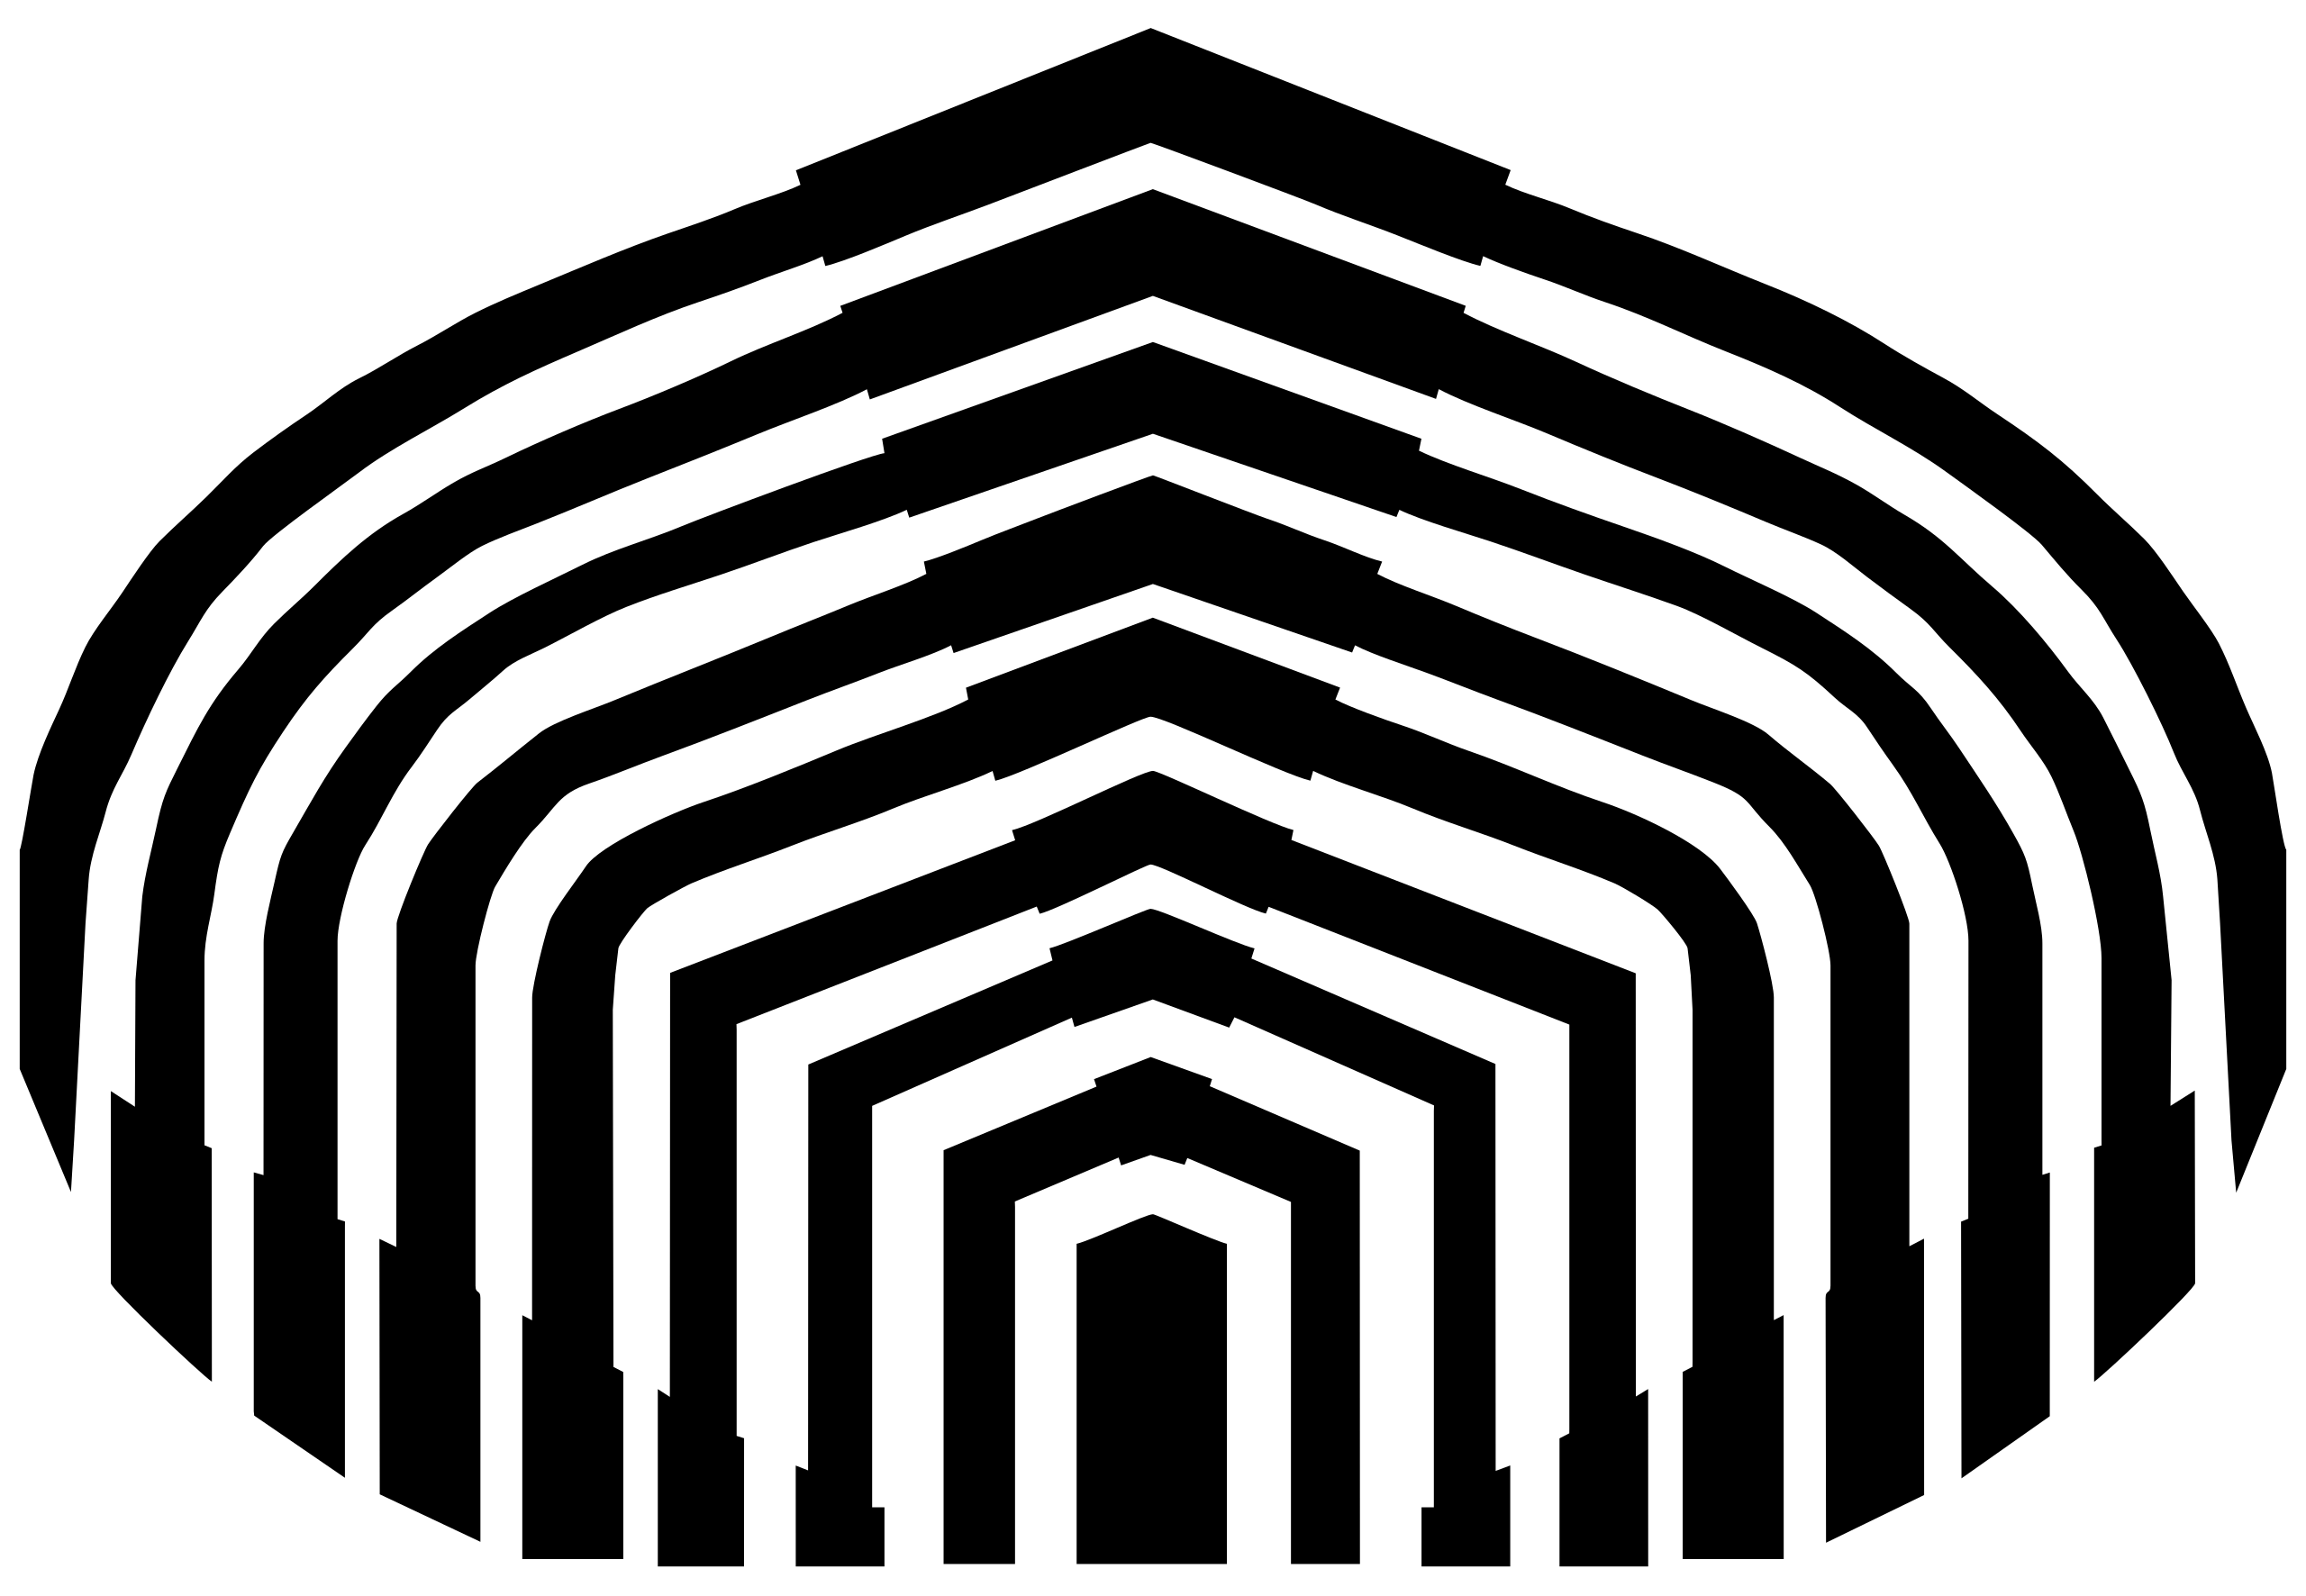
\includegraphics[width=3.1cm,height=2cm]{logo}\\
		UNIVERSIDAD SIMÓN BOLÍVAR\\
		DEPARTAMENTO DE ELECTRÓNICA Y CIRCUITOS\\
		EC1281 - LABORATORIO DE MEDICIONES ELÉCTRICAS\\
		SECCIÓN 1 - GRUPO 1\\
		
		\vspace{6cm}
		\textbf{\Large INFORME - PRÁCTICA \#8}\\
		EL VATIMETRO DIGITAL Y CARACTERÍSTICAS DEL TRANSFORMADOR MONOFÁSICO\\
	\end{center}
	
	\begin{flushleft}
		\vspace{9cm}
		\hfill Integrantes:\\
		\hfill {\large Luis Becerra - 1910557}\\
		\hfill {\large Lorena Rojas - 1910469}\\
	\end{flushleft}
	
	\newpage
	
	\pagenumbering{Roman}
        \setcounter{page}{2}
	
	\begin{center}
		\textbf{\large RESUMEN}\\
	\end{center}
	
	Inserte resumen
	
	\newpage
	
	\begin{center}
		\textbf{\large ÍNDICE}\\
	\end{center}
	
	\noindent \textbf{RESUMEN} \hfill \textbf{II}\\
	\noindent \textbf{ÍNDICE} \hfill \textbf{III}\\
	\noindent \textbf{MARCO TEÓRICO} \hfill \textbf{1}\\
	\noindent \textbf{METEDOLOGÍA} \hfill \textbf{4}\\
	\noindent \textbf{RESULTADOS} \hfill \textbf{5}\\
	\noindent \textbf{ANÁLISIS DE RESULTADOS} \hfill \textbf{13}\\
	\noindent \textbf{CONCLUSIONES} \hfill \textbf{14}\\
	\noindent \textbf{BIBLIOGRAFÍA} \hfill \textbf{15}\\
	\noindent \textbf{ANEXOS} \hfill \textbf{16}\\
	
	\newpage
	
	\pagenumbering{arabic}
	
	\begin{center}
		\textbf{\large MARCO TEÓRICO}\\
	\end{center}
	
	\textbf{1. }\\
	
	Inserte inciso 1
	
	\begin{itemize}
		\item \textbf{Sub-elemento 1 del inciso } inserte lo que corresponda
		
	\end{itemize}

	\newpage
	
	\begin{center}
		\textbf{\large METODOLOGÍA}\\
	\end{center}
	
	Inserte metodología
	
	\newpage
	
	\begin{center}
		\textbf{\large RESULTADOS}\\
	\end{center}
	
	A continuación se presentan los resultados obtenidos durante el trabajo en el laboratorio:
	
	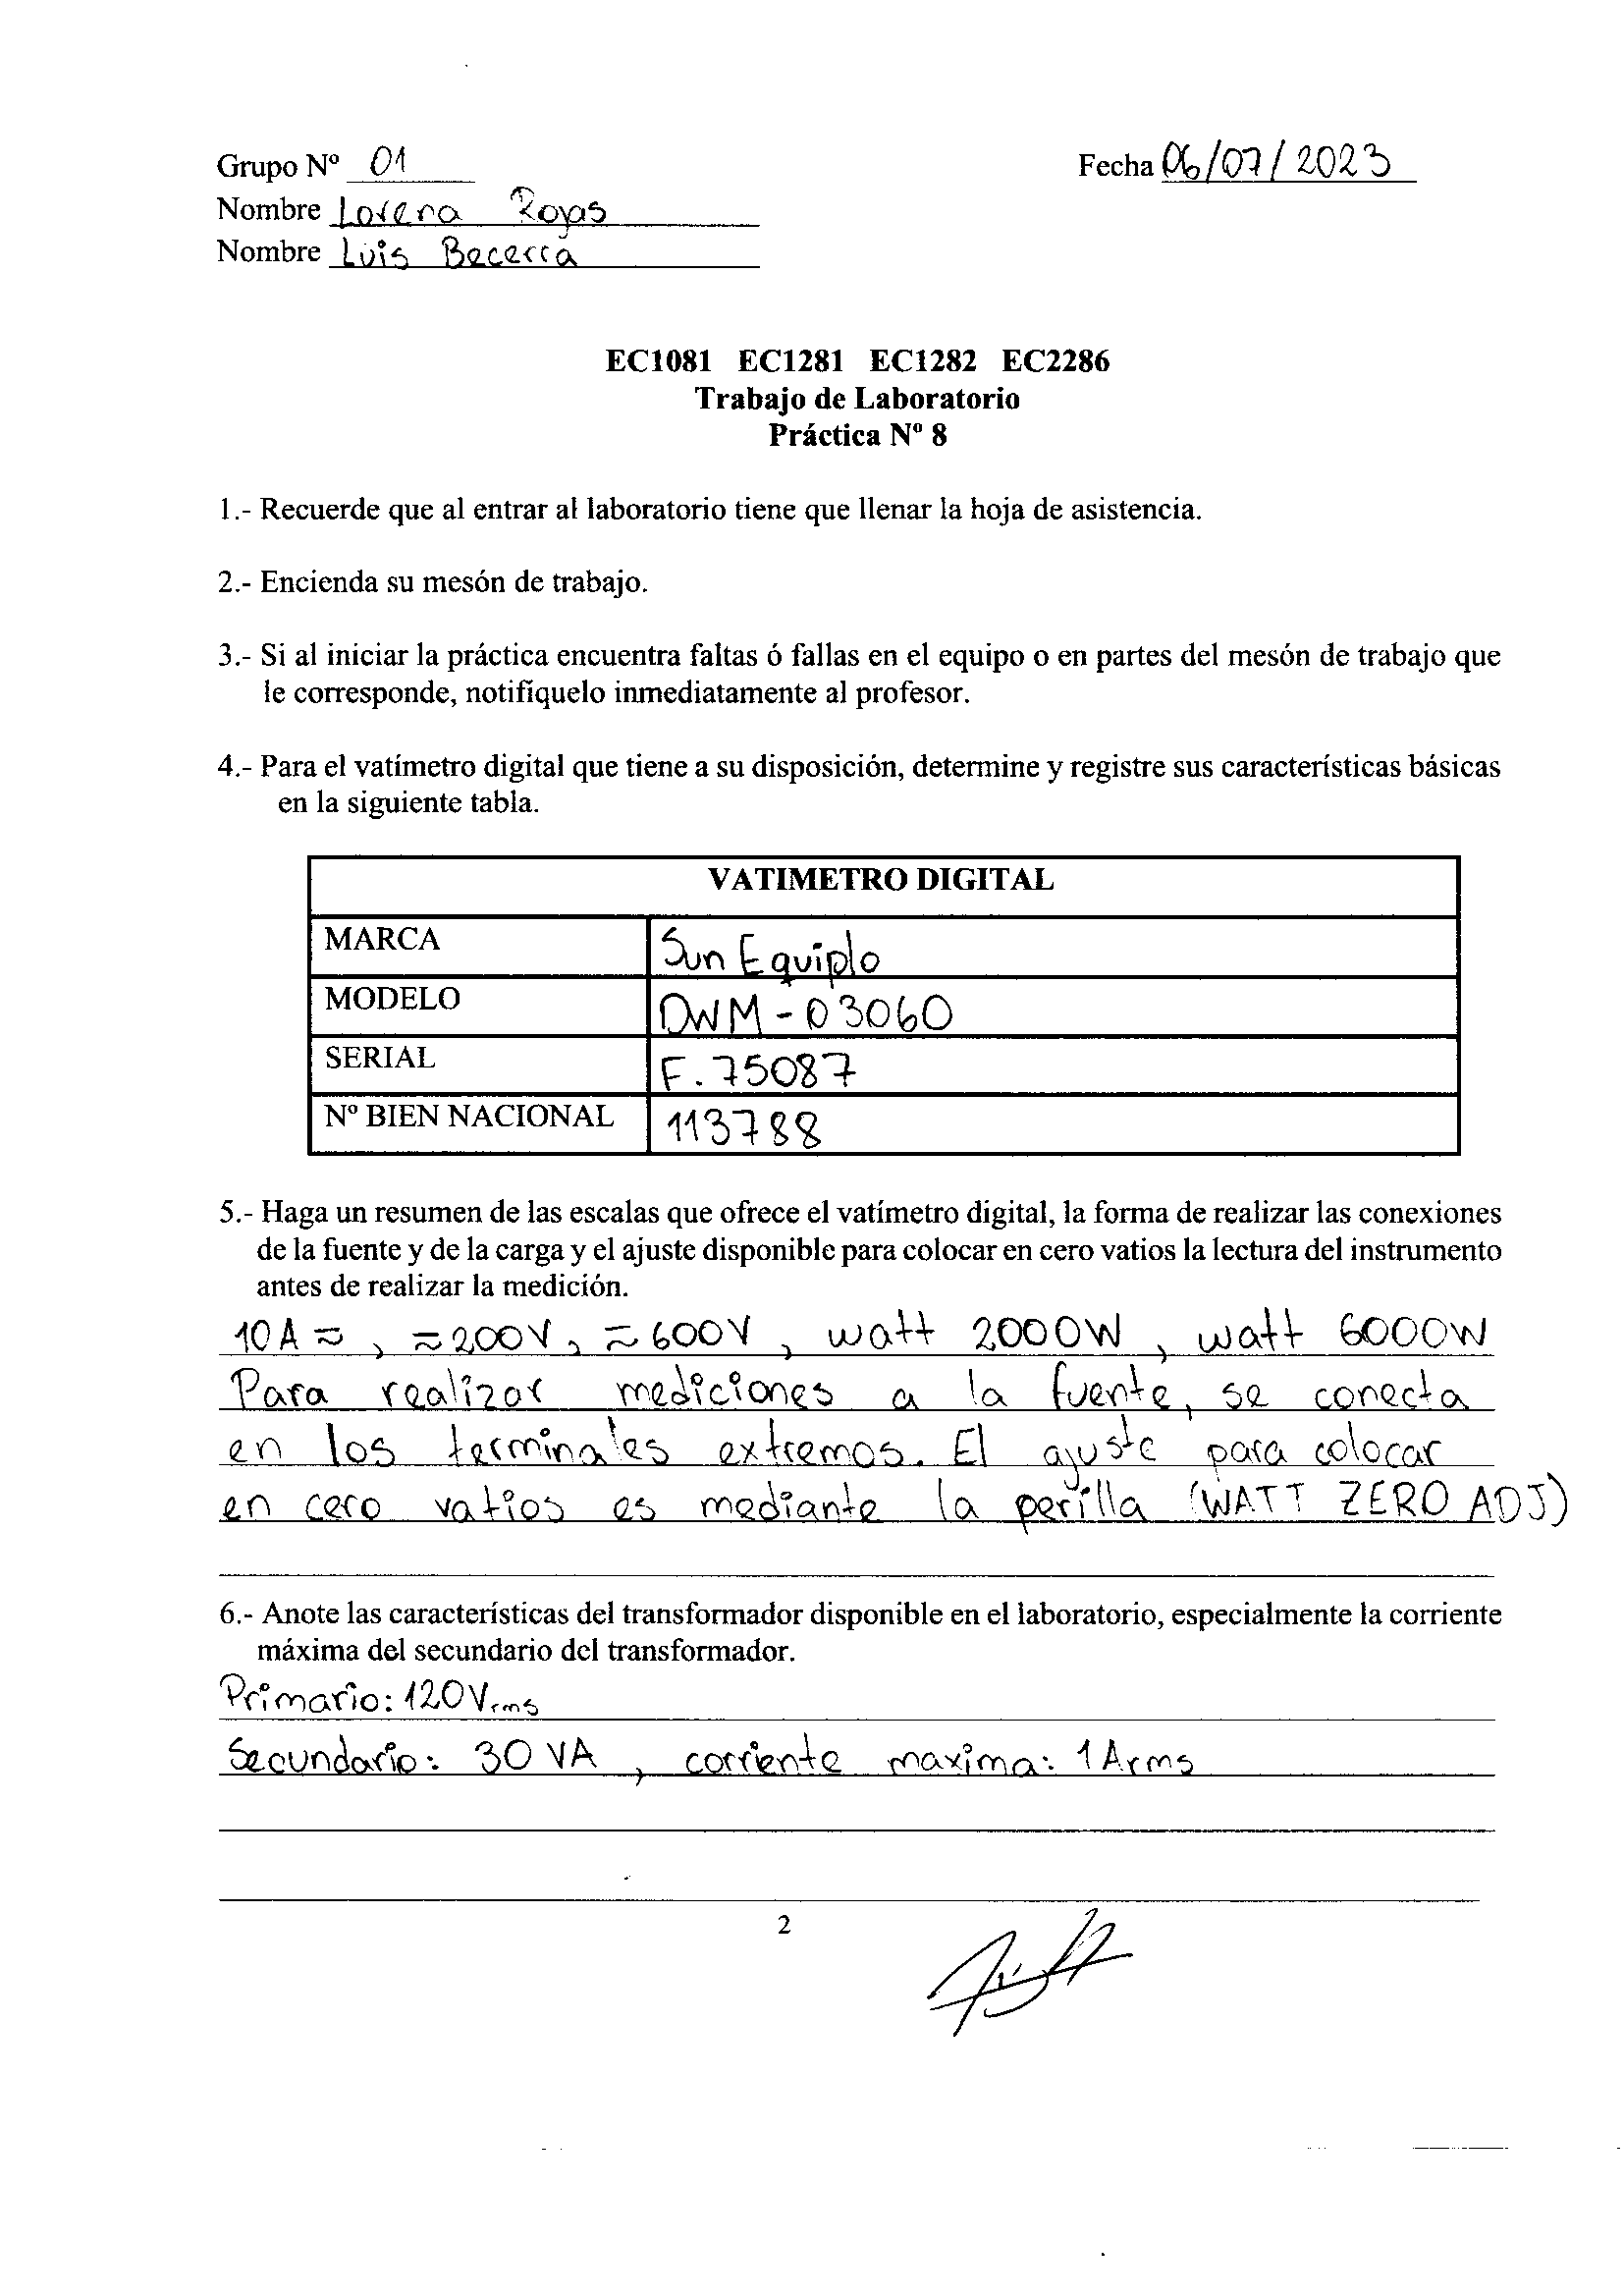
\includegraphics[width=16cm,height=21cm]{Img/lab_8_0001}\\
	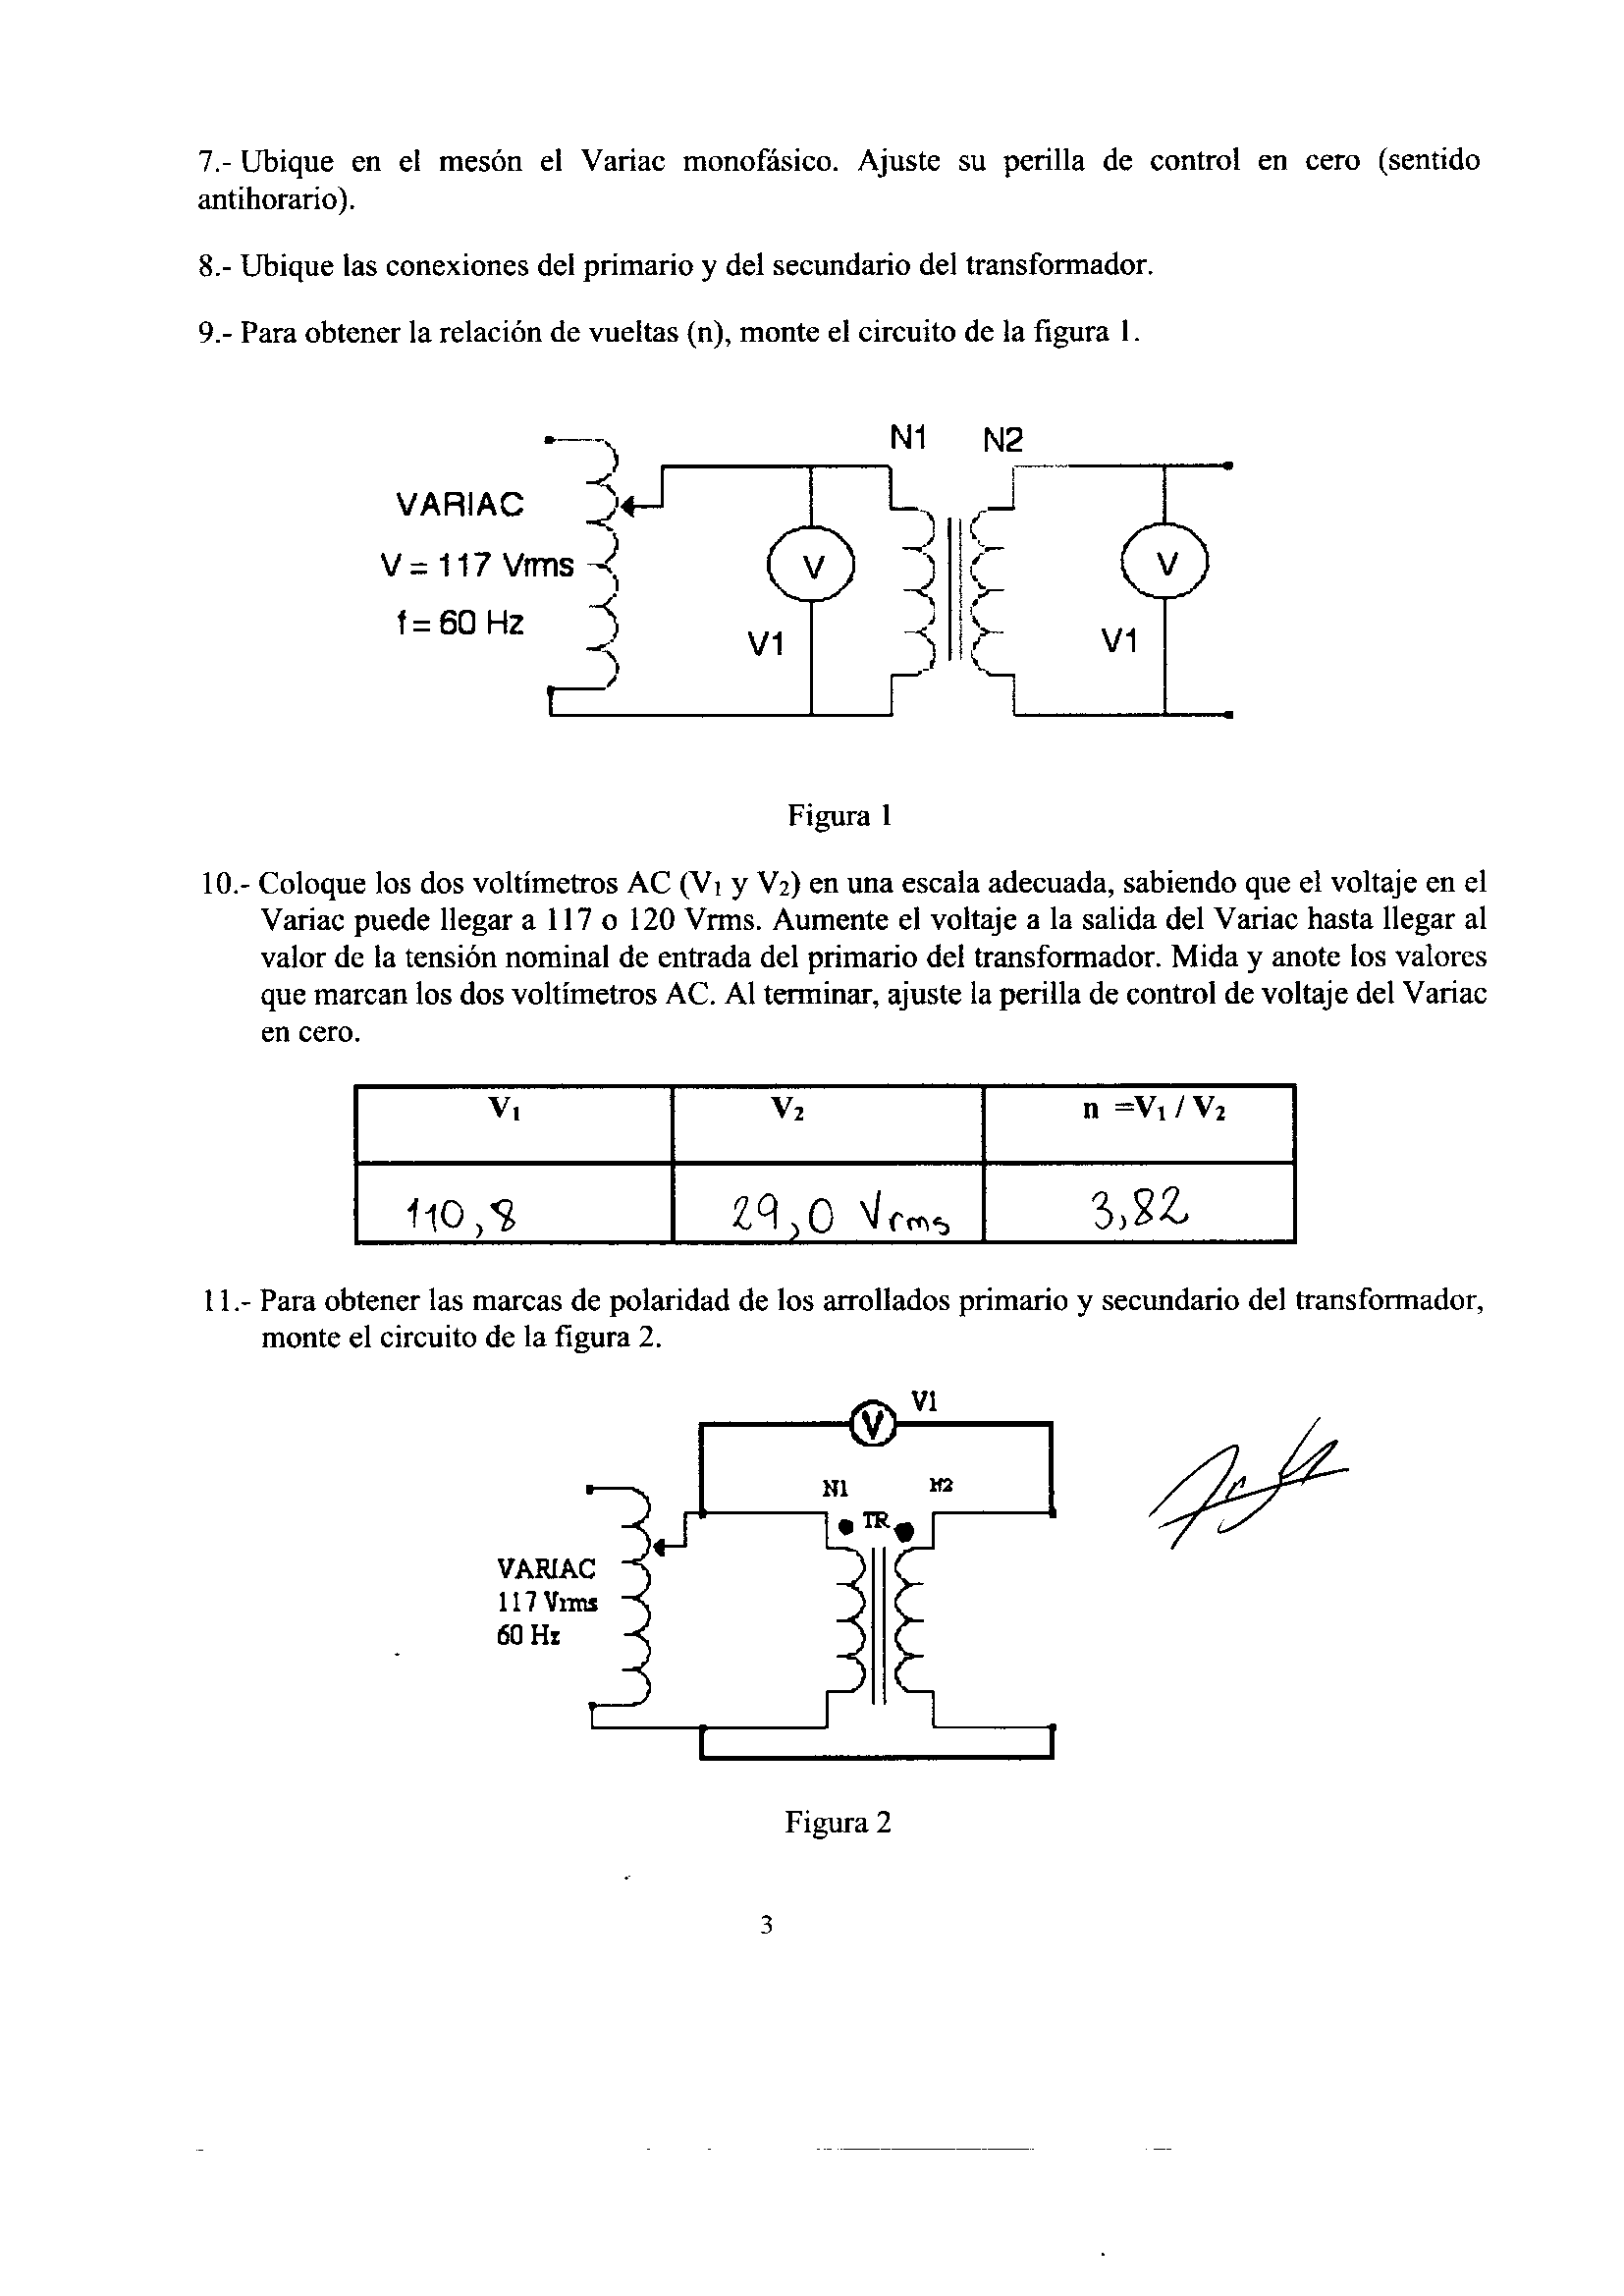
\includegraphics[width=16cm,height=21cm]{Img/lab_8_0002}\\
	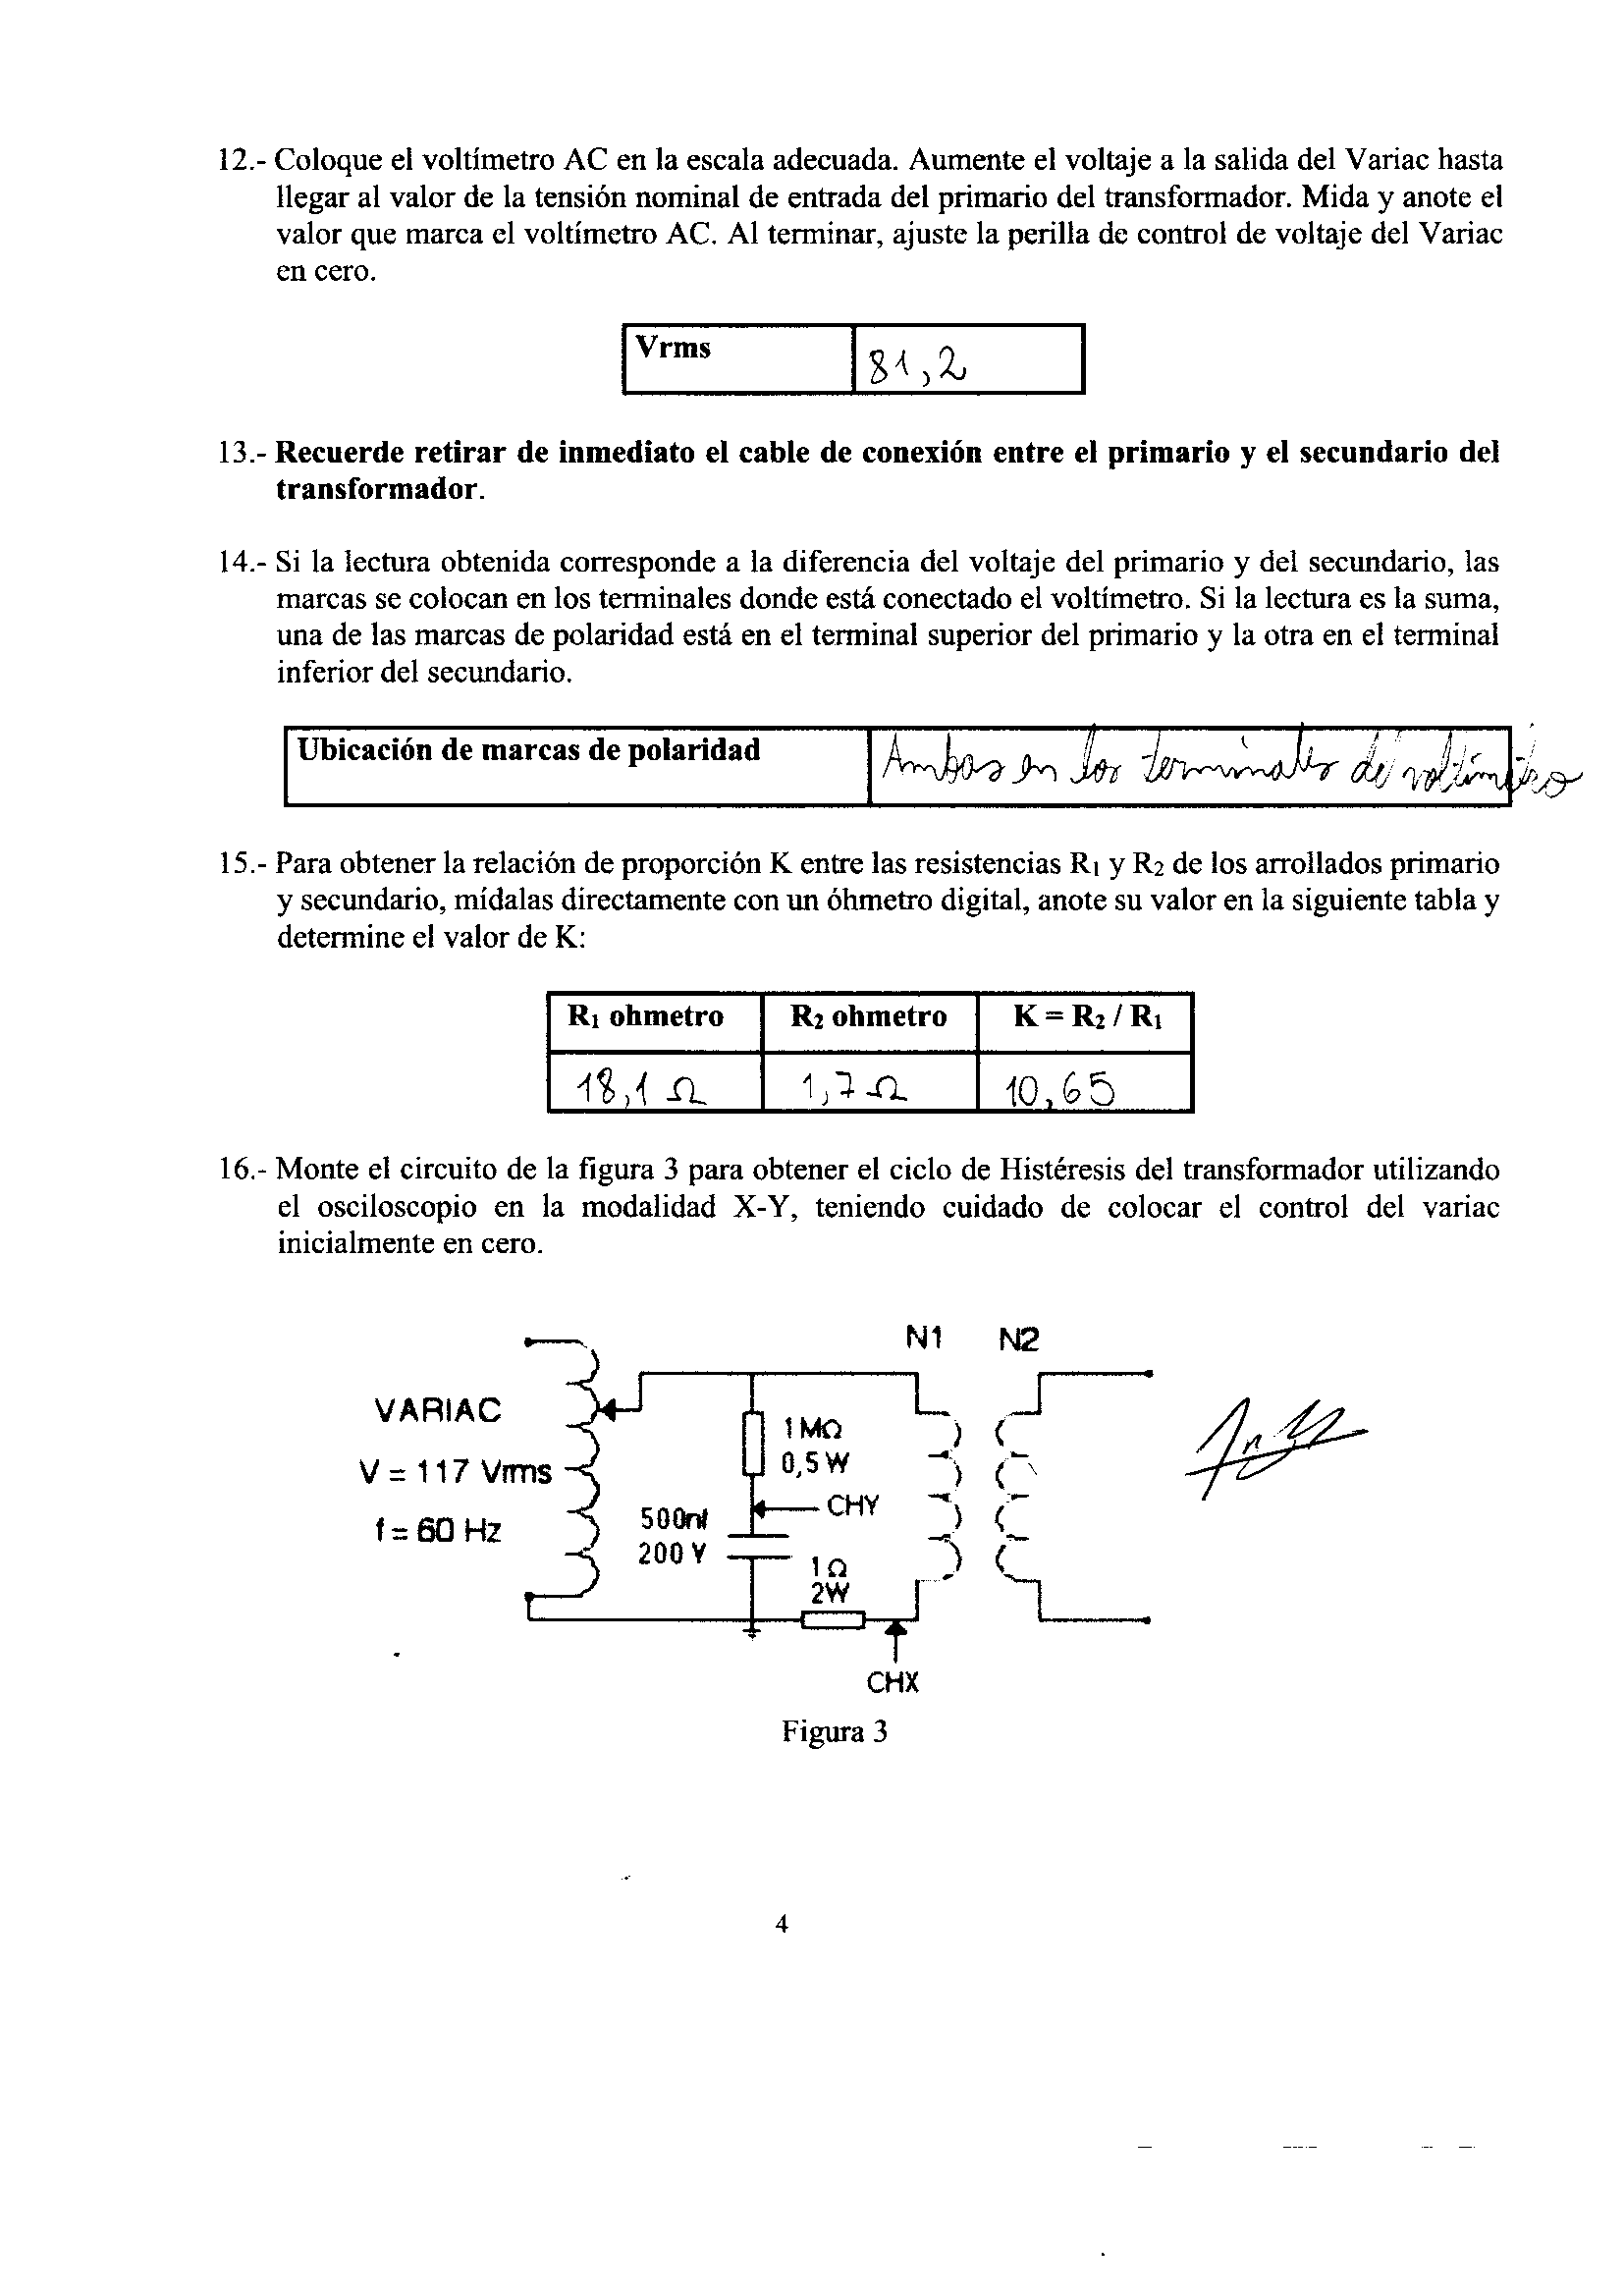
\includegraphics[width=16cm,height=21cm]{Img/lab_8_0003}\\
	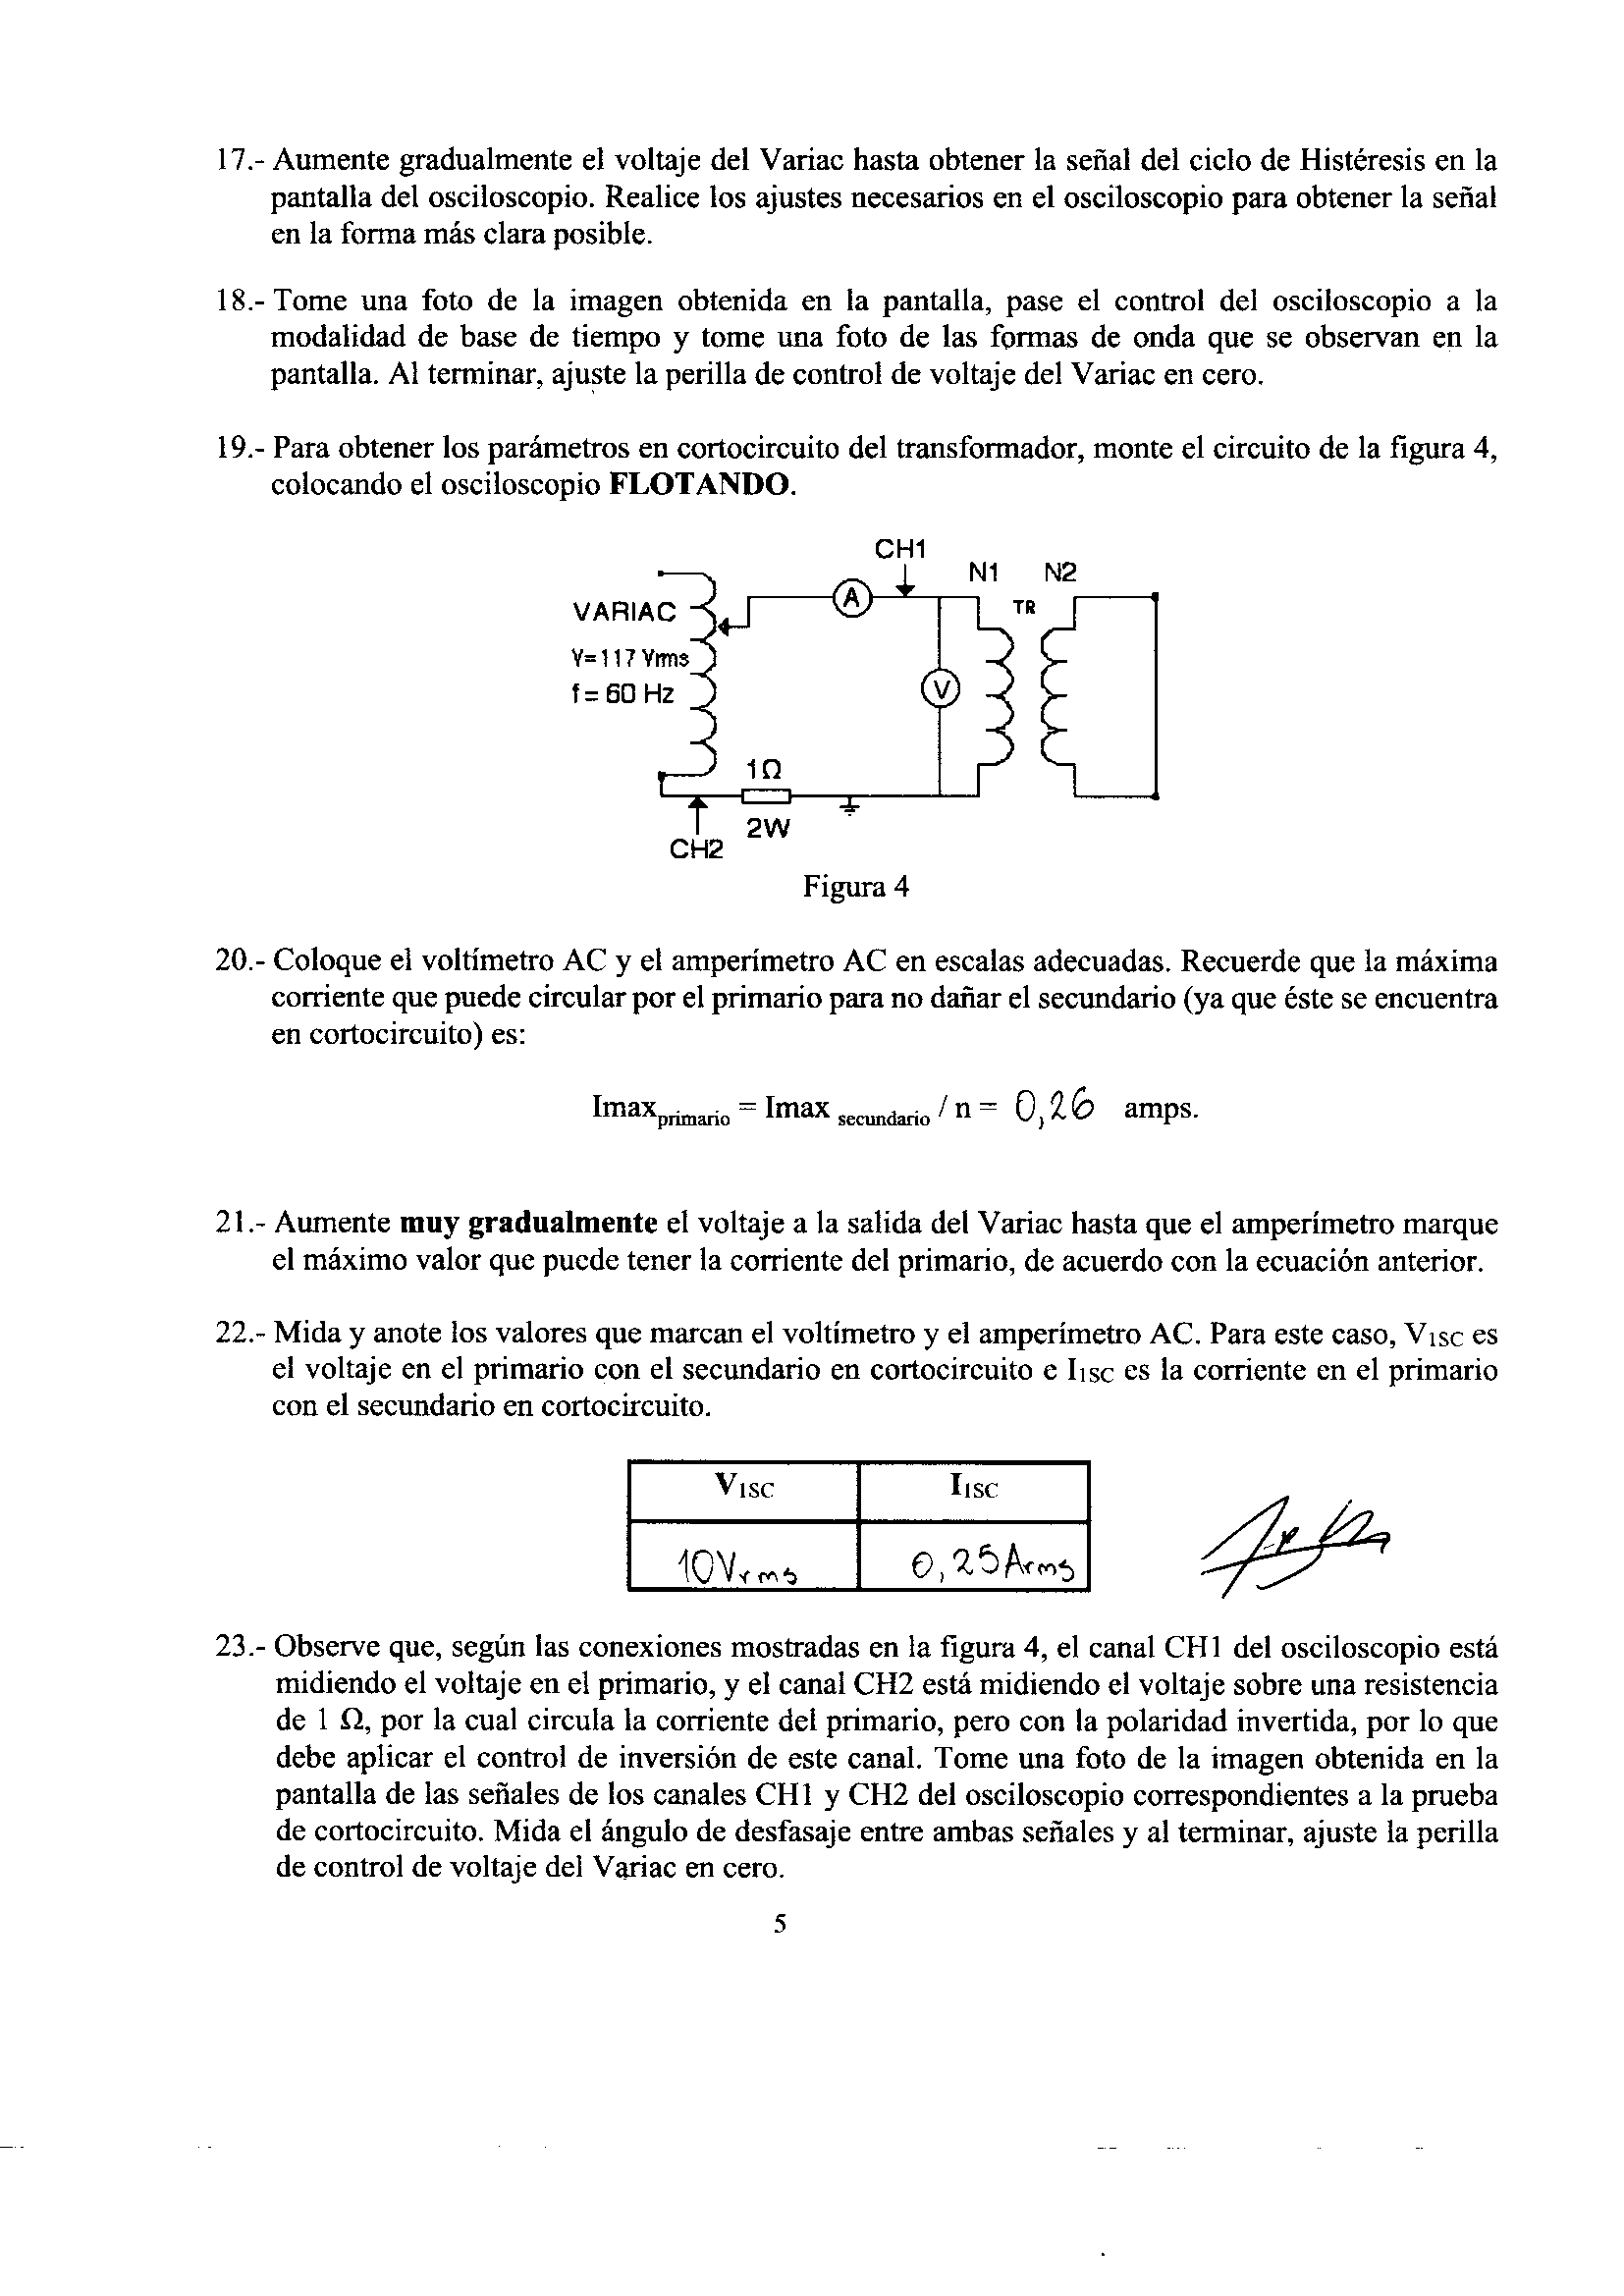
\includegraphics[width=16cm,height=21cm]{Img/lab_8_0004}\\
	
	\vspace{3cm}
	
	Respuesta a la pregunta 18:
	\begin{center}
		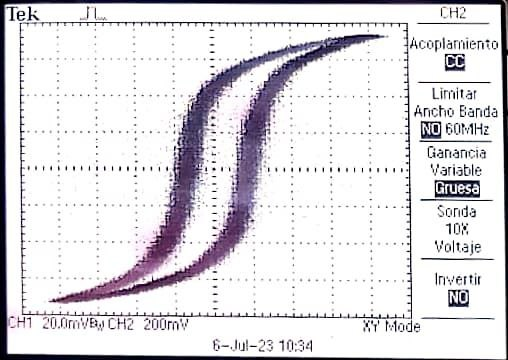
\includegraphics[width=8cm,height=6cm]{Img/figura1}\\
		\textit{Ciclo de Histeresis en la modalidad X-Y}
		
		\vspace{1cm}
		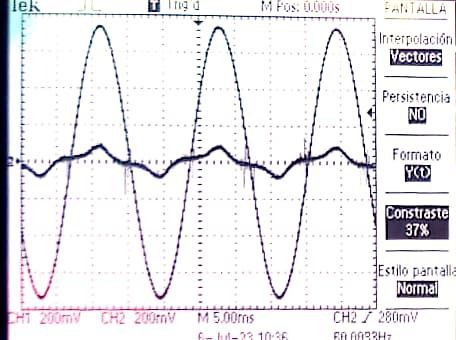
\includegraphics[width=8cm,height=6cm]{Img/figura2}\\
		\textit{Ciclo de Histeresis en función del tiempo}
		
		\vspace{1cm}
	\end{center}

	Respuesta a la pregunta 23:
	\begin{center}
		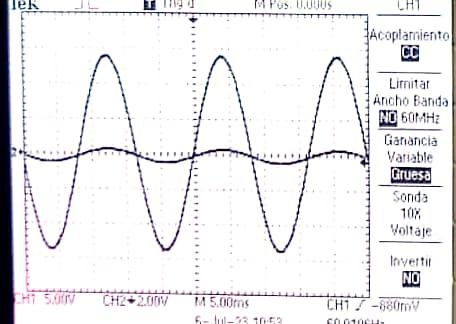
\includegraphics[width=8cm,height=6cm]{Img/figura3}\\
	\end{center}

	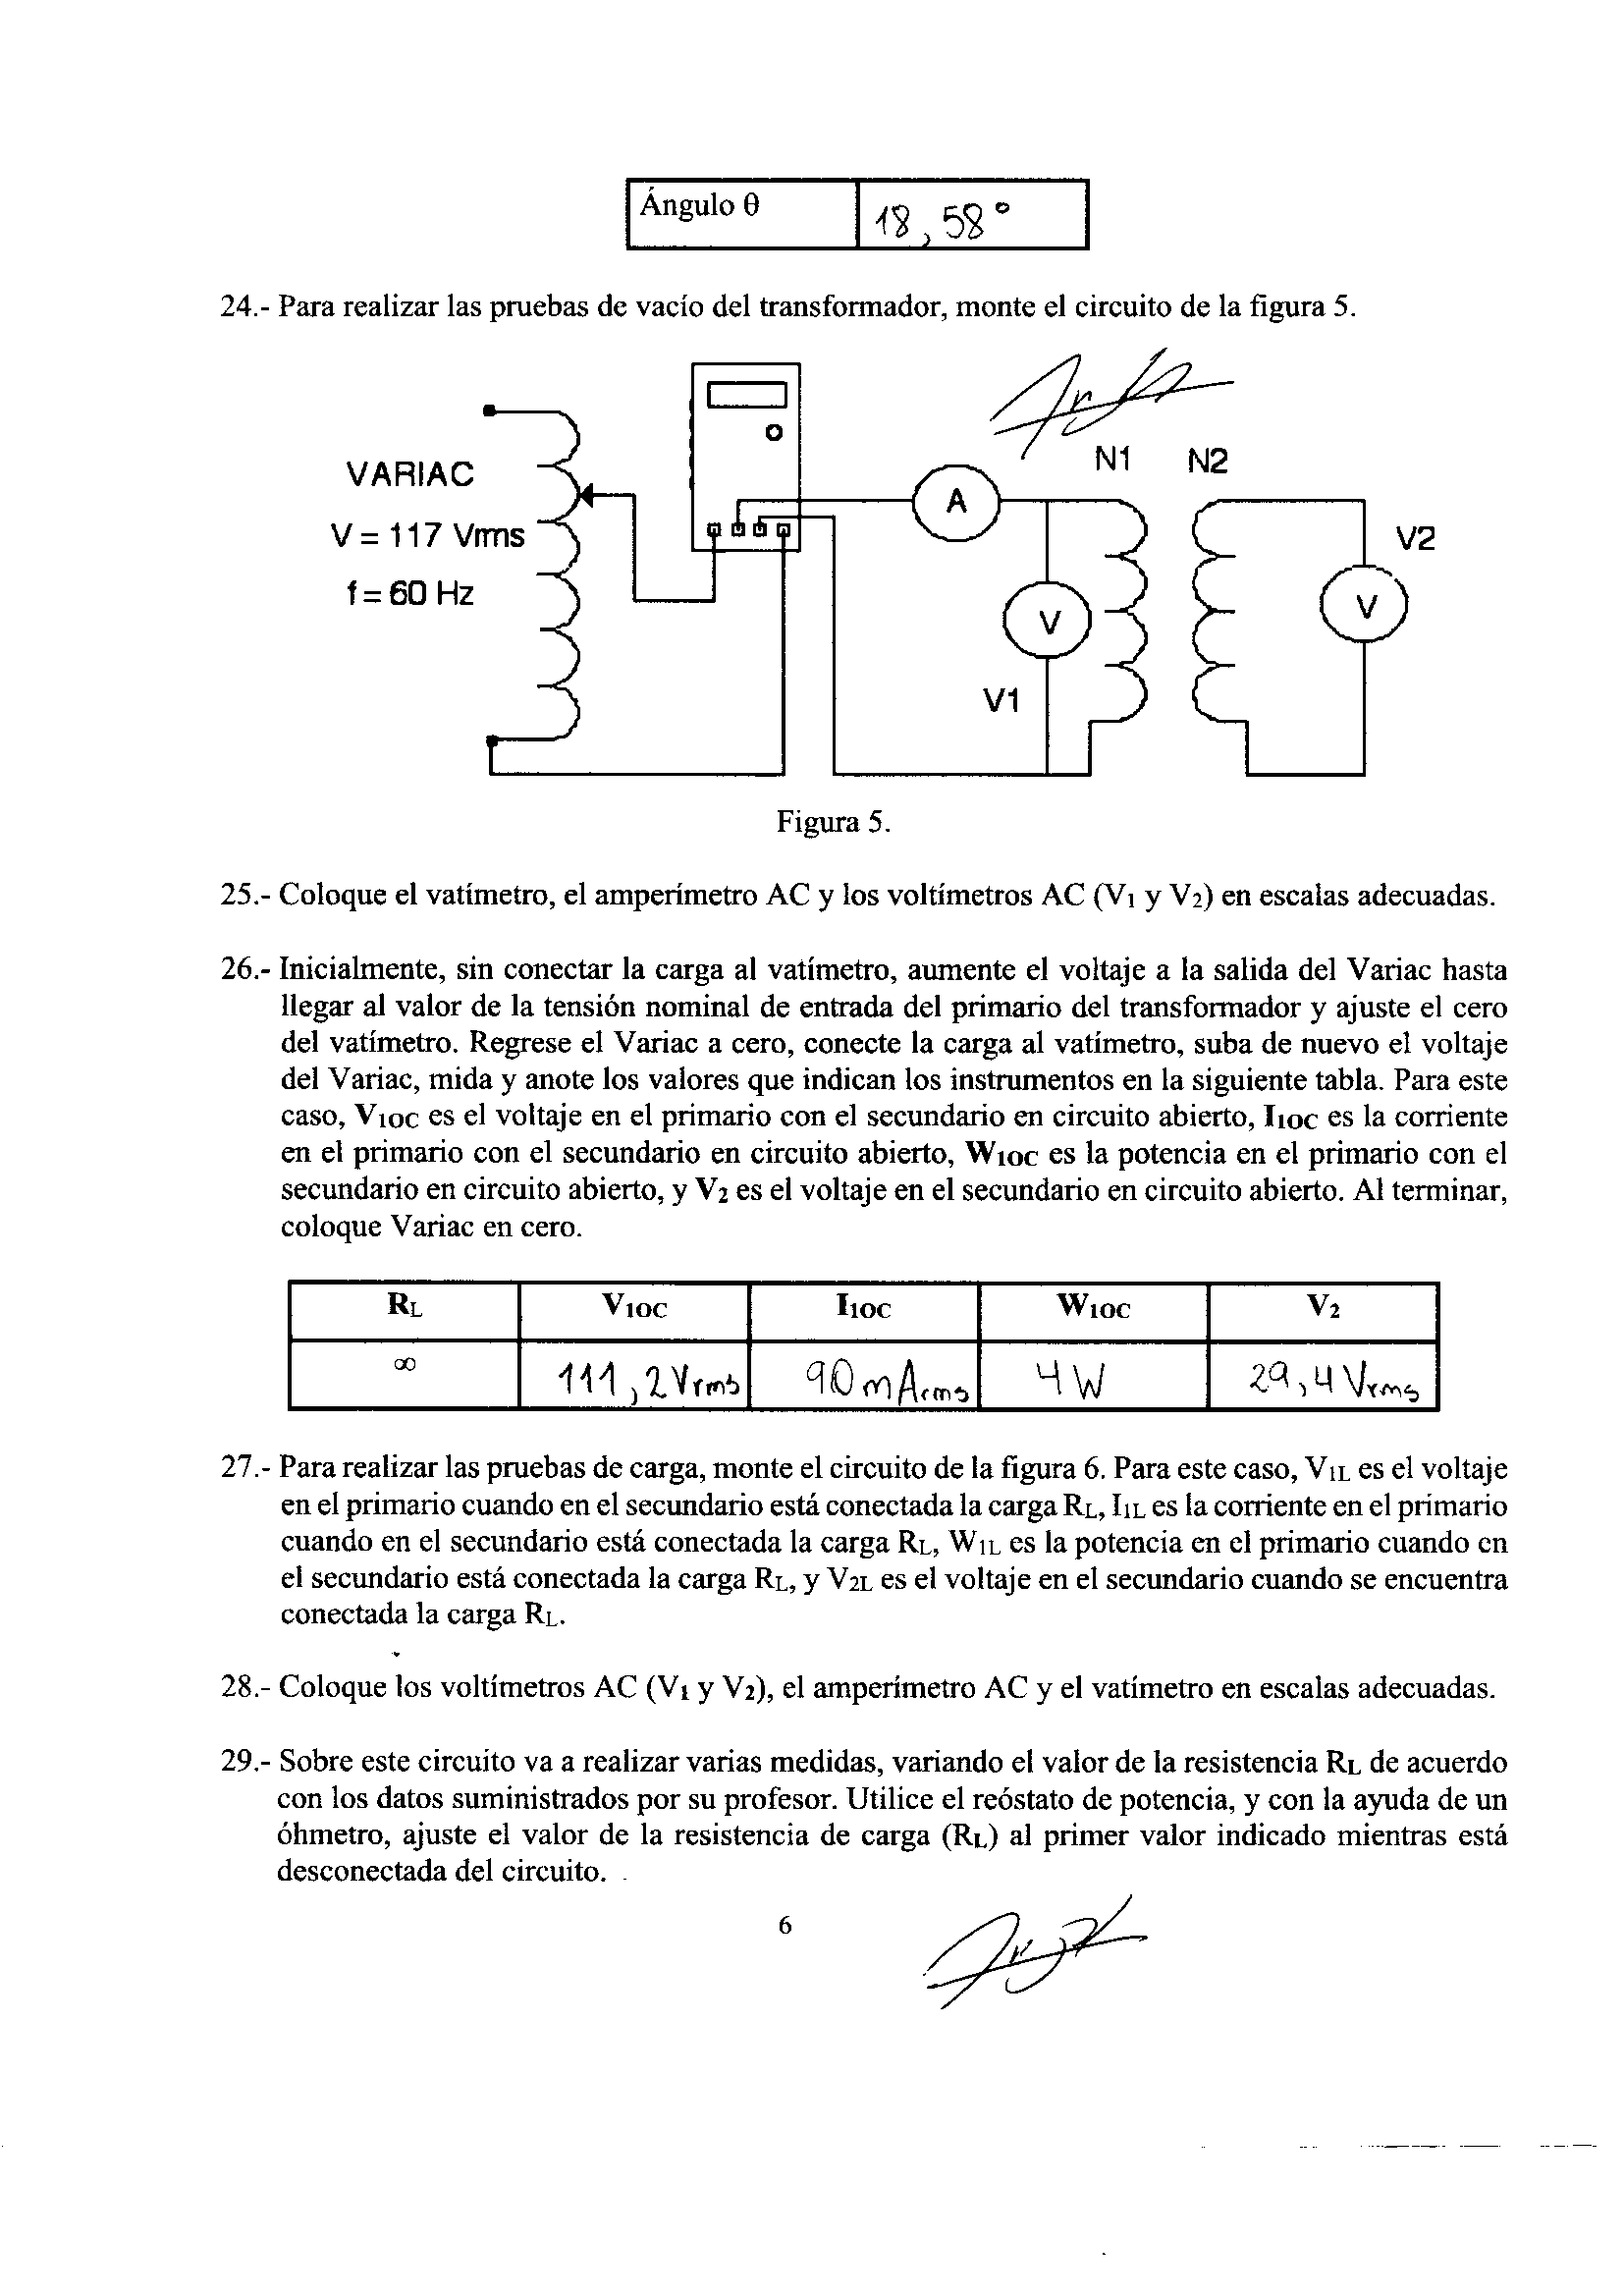
\includegraphics[width=16cm,height=21cm]{Img/lab_8_0005}\\
	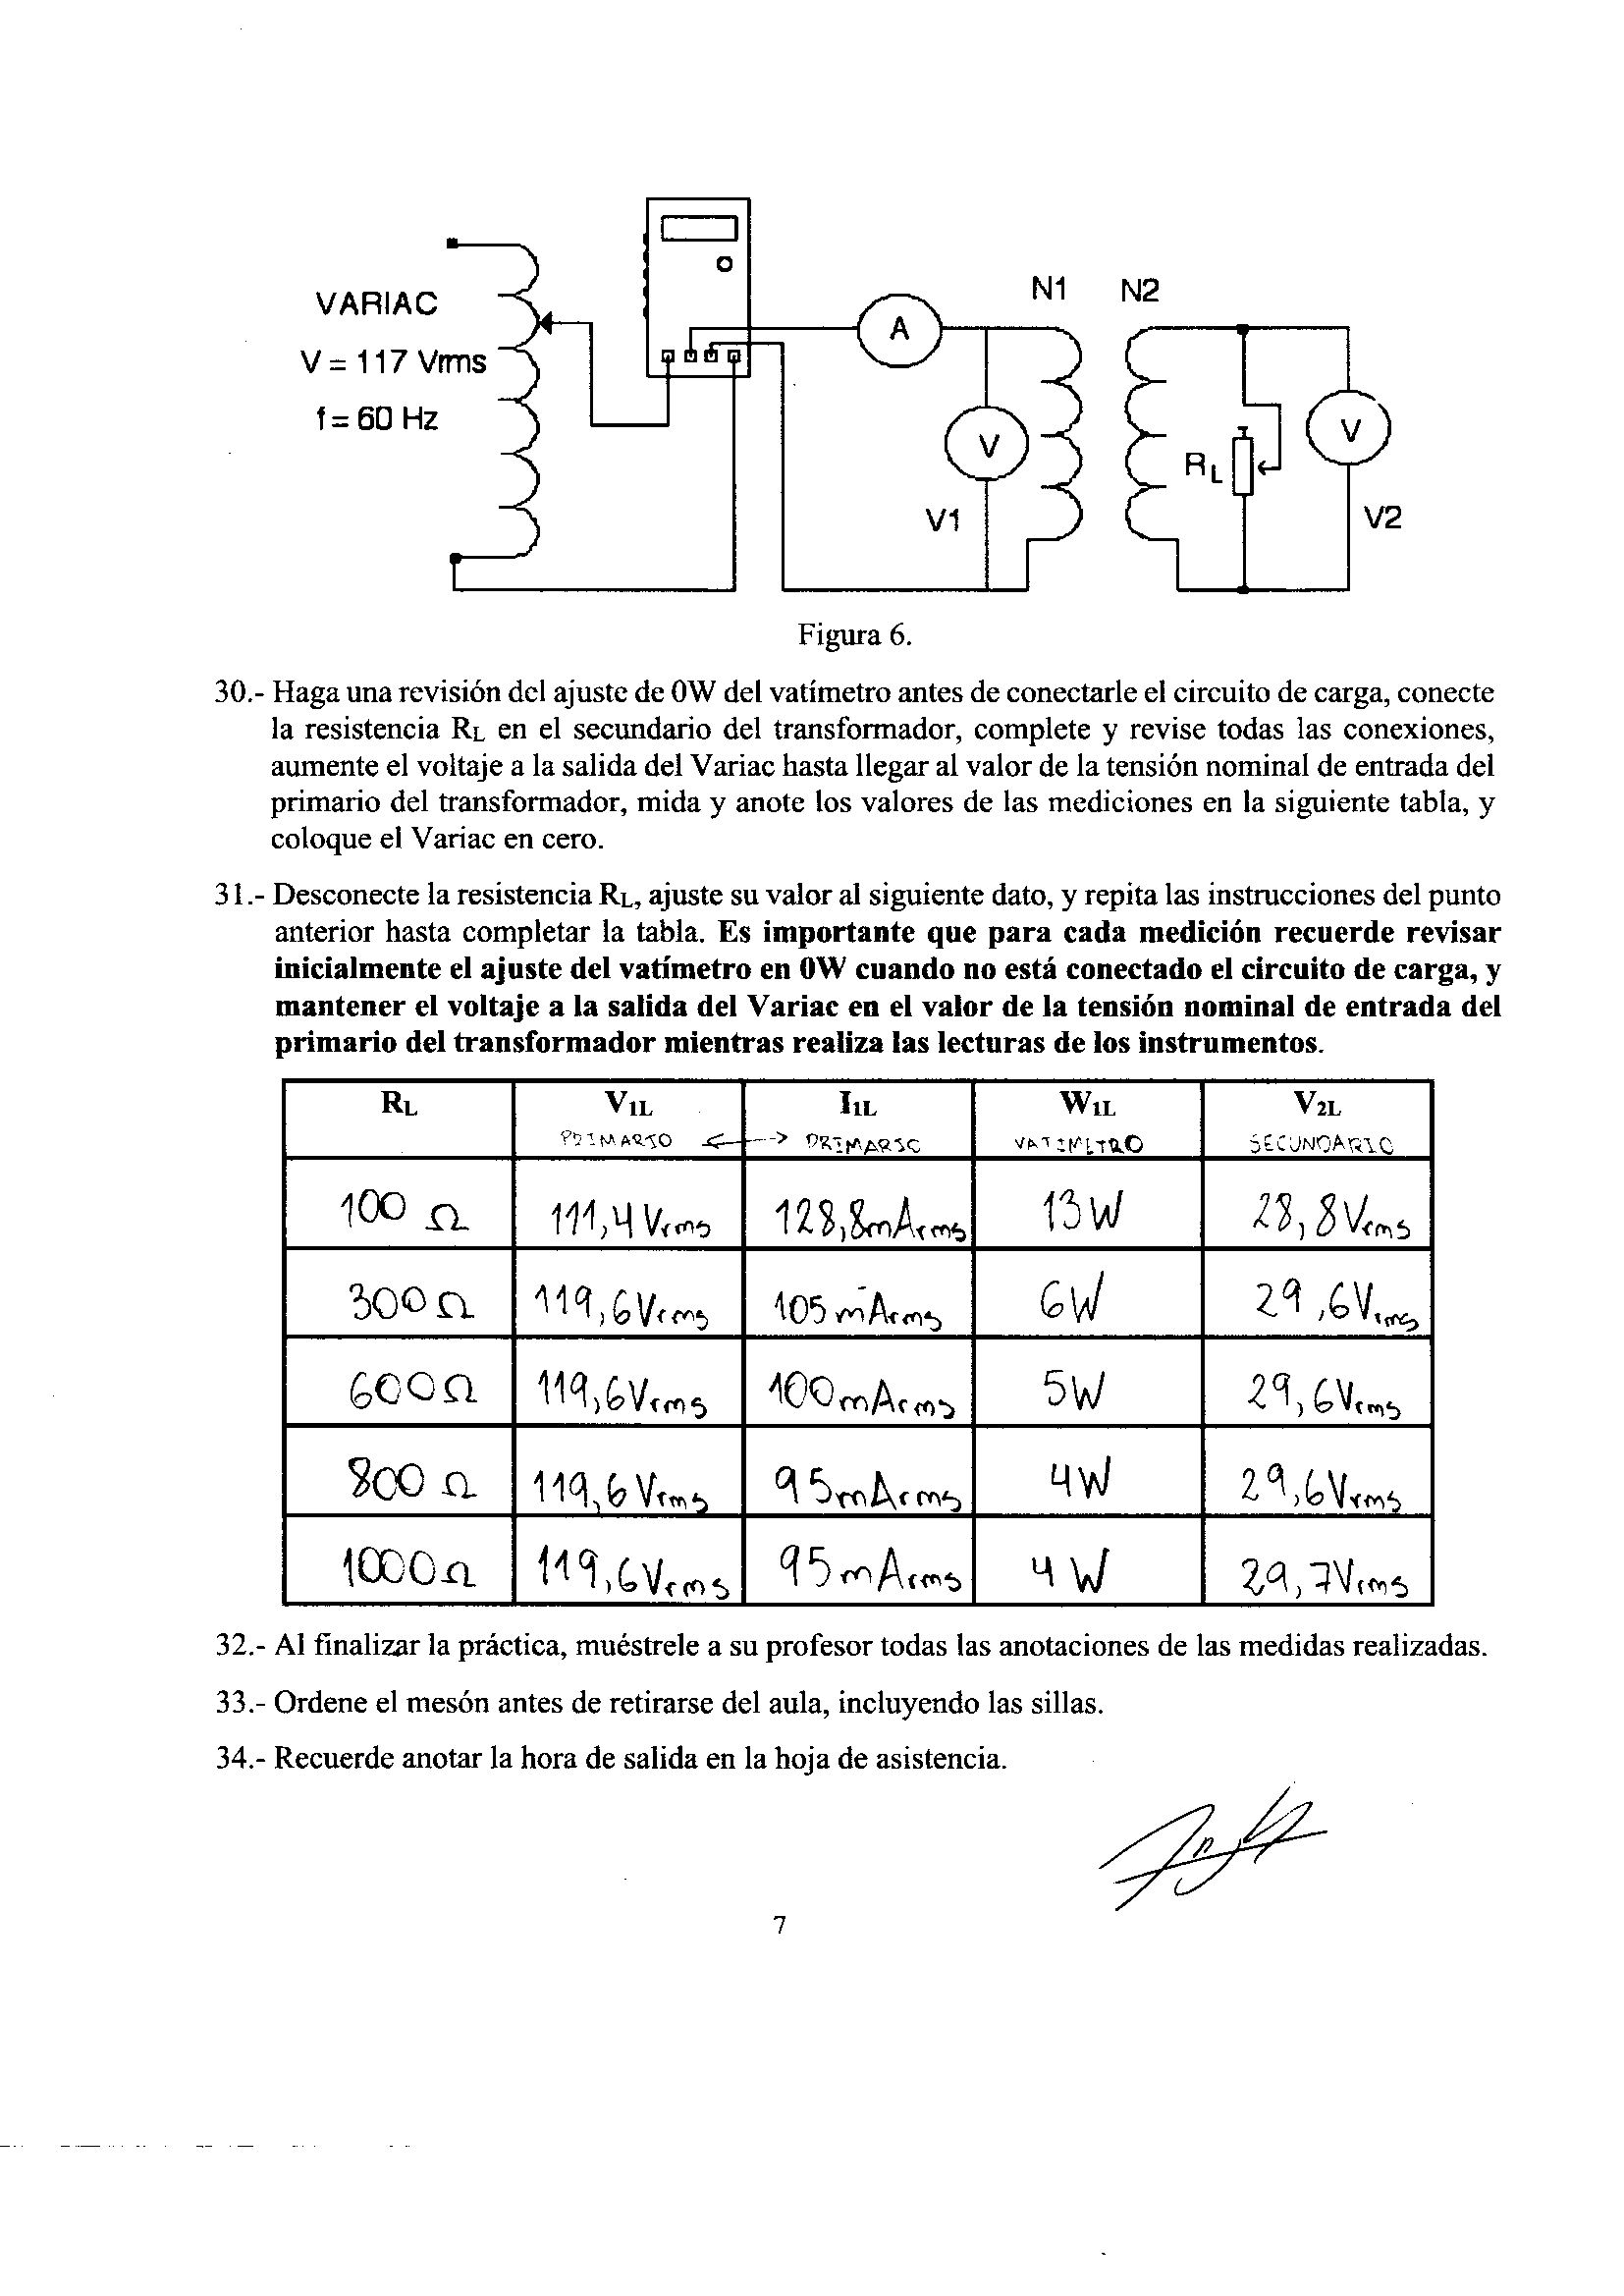
\includegraphics[width=16cm,height=21cm]{Img/lab_8_0006}\\
	
	\vspace{1cm}
	\noindent 1.- Con las mediciones realizadas durante la prueba de cortocircuito y los datos obtenidos en los experimentos anteriores (n y K) se calcula:\\
	
	a) La impedancia de entrada (módulo $|Z_{in}|= V_{1SC} / I_{1SC}$ y ángulo $\theta$).\\
	
	Con $V_{1SC} = 10 V_{rms}$, $I_{1SC} = 0,25 A_{rms}$ y $\theta = 18,58$ $$|Z_{in}| = \frac{10V_{rms}}{0,25A_{rms}} = 40 \Omega$$ $$Z_{in} = |Z_{in}|cos(\theta) + j|Z_{in}|sen(\theta) = 37,92 + j12,75$$
	
	b) Las resistencias de los dos devanados. Considere que la parte real de la impedancia de entrada, $|Z_{in}|cos(\theta)$, es igual a $R_{1} + n^2R_{2}$, donde $R_{2}$ es igual a $KR_{1}$.(Durante esta prueba la corriente de magnetización es muy pequeña, por lo	que la impedancia de magnetización se considera infinita).
	
	Con $n = 3,82$ y $K = 10,65$ $$|Z_{in}|cos(\theta) = R_{1} + n^2KR_{1} \Rightarrow R_{1} = \frac{|Z_{in}|cos(\theta)}{1 + n^2K} = \frac{37,92}{156,41} \Omega= 0,24\Omega$$ $$R_{2} = KR_{1} = 2,58 \Omega$$
	
	c) La reactancia de dispersión de los dos devanados. Considere que la parte imaginaria	de la impedancia de entrada, $|Z_{in}|sen(\theta)$, es igual a $X_{1} + n^2X_{2}$, donde $X_{2}$ es igual a $KX_{1}$. $$|Z_{in}|sen(\theta) = X_{1} + n^2KX_{1} \Rightarrow X_{1} = \frac{|Z_{in}|sen(\theta)}{1 + n^2K} = \frac{12,75}{156,41} \Omega = 0,08 \Omega$$ $$X_{2} = KX_{1} = 0,87 \Omega$$
	
	d) Las inductancias de dispersión de los dos devanados, $L_{1}$ y $L_{2}$ $(L = X/2 \pi f)$. $$L_{1} = \frac{X_{1}}{2\pi f} = 0,2 mH$$  $$L_{2} = \frac{X_{2}}{2\pi f} = 2,3 mH$$ 
	
	e) Las pérdidas en el cobre $(P_{cu})$. Ecuación : $P_{cu} = (I_{prim.(sc)})^2(R_{1} + n^2R_{2})$. \\
	
	Donde $I_{\textit{prim(sc)}} = 0.25A$ es la corriente primaria de cortocircuito, entonces: $$P_{cu} = (0,25)^2 \cdot (0,24 + (3,82)^2 \cdot (2,58)) = 2,34 W$$
	
	\noindent 2.- Con las mediciones realizadas durante la prueba de circuito abierto calcule:\\
	
	a) El factor de potencia en vacío $f_{p} = W_{1OC}/(V_{1OC} I_{1OC}$). \\
	
	Con $V_{1OC} = 111,2 V_{rms}$, $I_{1OC} = 90 m A_{rms}$ y $W_{1OC} = 4 W$
	$$f_{p} = \frac{4W}{111,2 V_{rms} \cdot 90 m A_{rms}} = 0.40$$
	b) La resistencia de pérdidas magnéticas $R_{p} = V_{1OC}^2 /W_{1OC}$. $$R_{p} = \frac{(111,2 V_{rms})^2}{4W} = 3091,36 \Omega$$
	c) La corriente de pérdidas $I_{p} = V_{1OC}/ R_{p}$. $$I_{p} = \frac{111,2 V_{rms}}{3091,36 \Omega} = 0,036 A$$
	d) La corriente de magnetización $I_{m} = \sqrt{(I_{1OC}^2 - I_{p}^2)}$. $$I_{m} = \sqrt{(90 m A_{rms})^2 - (0,036 A)^2} = 0,0825 A$$
	e) La reactancia de magnetización $X_{m} = V_{1OC}/ I_{m}$. $$X_{m} = \frac{111,2 V_{rms}}{0,0825 A} = 1347,88 \Omega$$
	f) La inductancia de magnetización $L_{m} = X_{m}/2\pi f$. $$L_{m} = \frac{1347,88 \Omega}{2\pi(60Hz)} = 3,58 H$$
	
	\noindent 3.- Con los datos obtenidos durante la prueba de carga, elabore los siguientes gráficos:\\
	
	a) Potencia de entrada vs. resistencia de carga (RL).\\
	
	\begin{center}
		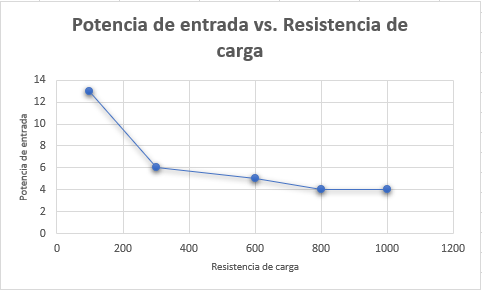
\includegraphics[width=12cm,height=8cm]{Img/grafo1}\\
	\end{center}
	
	b) Corriente de entrada vs. resistencia de carga (RL).\\
	
	\begin{center}
		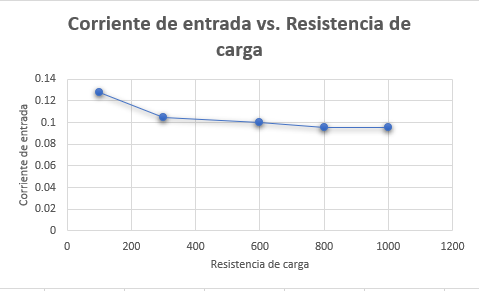
\includegraphics[width=12cm,height=8cm]{Img/grafo2}\\
	\end{center}
	
	c) Voltaje en el secundario vs. resistencia de carga (RL).\\
	
	\begin{center}
		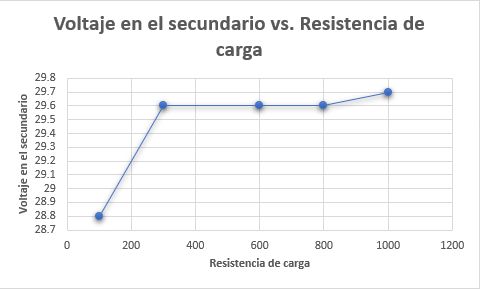
\includegraphics[width=12cm,height=8cm]{Img/grafo3}\\
	\end{center}
	
	\noindent 4.- Calcule el valor de la regulación de voltaje (h) en el secundario aplicando la siguiente	fórmula: $$n = (\frac{V_{secundario(vacio)} - V_{secundario(plena carga)}}{V_{secundario(vacío)}}) \cdot 100\%$$
	
	Con $V_{secundario(vacio)} = V_{2} = 29,4 V_{rms}$ y $V_{secundario(plena carga)} = V_{2L} = 28,8 V_{rms}$ $$n = (\frac{29,4 V_{rms} - 28,8 V_{rms}}{29,4 V_{rms}}) \cdot 100\% = 2,04\% $$
	
	Con $V_{secundario(vacio)} = V_{2} = 29,4 V_{rms}$ y $V_{secundario(plena carga)} = V_{2L} = 29,6 V_{rms}$ $$n = (\frac{29,4 V_{rms} - 29,6 V_{rms}}{29,4 V_{rms}}) \cdot 100\% = 0,68\% $$
	
	Con $V_{secundario(vacio)} = V_{2} = 29,4 V_{rms}$ y $V_{secundario(plena carga)} = V_{2L} = 29,7 V_{rms}$ $$n = (\frac{29,4 V_{rms} - 29,7 V_{rms}}{29,4 V_{rms}}) \cdot 100\% = 1,02\% $$
		
	\newpage
	
	\begin{center}
		\textbf{\large ANÁLISIS DE RESULTADOS}\\
	\end{center}
	
	a) Haga un diagrama completo del modelo circuital del transformador, indicando el valor calculado para cada uno de los parámetros.\\
	
	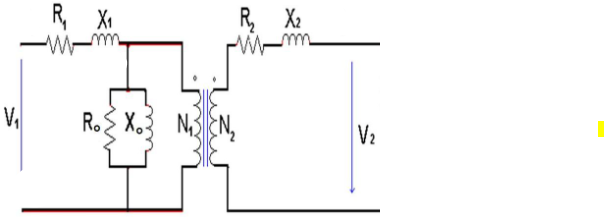
\includegraphics[width=22cm,height=6cm]{Img/transformador}\\
	$$R_{o} = R_{p} = 3091,36 \Omega$$
	$$R_{1} = 0,24 \Omega$$
	$$R_{2} = 2,58 \Omega$$
	$$X_{o} = L_{m} = 3,58 H$$
	$$X_{1} = L_{1} = 0,2 mH$$
	$$X_{2} = L_{2} = 2,3 mH$$
	
	b) Analice los resultados obtenidos y haga comentarios sobre las aproximaciones realizadas.
	
	Al analizar las gráficas construidas a partir de las pruebas de carga, se pueden obtener conclusiones más detalladas sobre el comportamiento del transformador monofásico. A continuación, se presenta un análisis:\\
	
	\begin{itemize}
		\item Se observa que la potencia y la corriente de entrada disminuyen a medida que la resistencia de carga aumenta. Esto se debe a la relación entre el voltaje, la corriente y la resistencia según la ley de Ohm. Al aumentar la resistencia de carga, la corriente que fluye a través del circuito disminuye, lo que a su vez reduce la potencia de entrada. Esto implica que el transformador es capaz de adaptarse a diferentes cargas y suministrar la potencia requerida de manera eficiente.
		
		\item Además, se puede notar que el voltaje en el secundario aumenta proporcionalmente al valor de la resistencia de carga. Esto se debe a que el transformador está diseñado para mantener una relación de voltaje constante entre el primario y el secundario. Al aumentar la resistencia de carga, se produce una mayor caída de voltaje en la resistencia, lo que resulta en un aumento del voltaje en el secundario del transformador.
		
		\item Es importante destacar que el transformador tiene límites de corriente máxima tanto en el primario como en el secundario. Esto es crucial al diseñar circuitos que utilicen este componente, ya que se debe garantizar que la corriente no exceda los límites especificados para evitar daños al transformador y garantizar su funcionamiento seguro y eficiente.
		
		\item Además, es relevante considerar la eficiencia del transformador al seleccionar la carga óptima. La eficiencia máxima se logra cuando la potencia de salida es la máxima posible para una potencia de entrada determinada. Esto garantiza un uso eficiente de la energía y minimiza las pérdidas en el transformador.
		
		\item Otros aspectos a tener en cuenta en el diseño de circuitos con transformadores incluyen la caída de voltaje, que puede afectar la calidad de la señal, y la impedancia del transformador, que debe ser compatible con la carga para una transferencia eficiente de energía. Además, la compensación de reactancia puede ser necesaria para corregir problemas de desfasaje y mejorar el rendimiento del circuito.
	\end{itemize}
	
	
	\newpage
	
	\begin{center}
		\textbf{\large CONCLUSIONES}\\
	\end{center}
	
	En conclusión, a partir del desarrollo de este laboratorio y las mediciones experimentales realizadas, se puede afirmar lo siguiente: \\
	
	Es sumamente útil poder conocer en detalle mediante mediciones experimentales el modelo circuital de un transformador real. Esto nos brinda información precisa sobre sus parámetros y características, lo que nos permite comprender mejor su comportamiento en diferentes condiciones de carga. Conocer el modelo circuital del transformador nos ayuda a diseñar y dimensionar adecuadamente circuitos que lo incluyan, asegurando un funcionamiento eficiente y seguro.\\
	
	Los vatímetros desempeñan un papel fundamental en la aplicación de las pruebas para conocer los parámetros del transformador. Gracias a ellos, podemos medir con precisión la potencia y la corriente en el transformador, lo que nos permite determinar sus características de rendimiento y eficiencia. Los vatímetros digitales utilizados en este laboratorio ofrecen una forma precisa y confiable de medir y registrar estos valores, facilitando así el análisis y la interpretación de los datos.\\
	
	La obtención del ciclo de histéresis de un transformador real en la pantalla del osciloscopio resulta de gran utilidad. Esta prueba nos permite analizar el comportamiento magnético del transformador, especialmente en lo que respecta a la histéresis y la pérdida de energía asociada. Al visualizar el ciclo de histéresis en el osciloscopio, podemos evaluar la eficiencia del transformador y realizar ajustes necesarios para optimizar su rendimiento.\\
	
	En general, este trabajo de laboratorio nos ha permitido adquirir conocimientos prácticos sobre el funcionamiento y las características de un transformador monofásico. A través de la preparación previa, las mediciones experimentales y el análisis de los datos, hemos podido comprender la importancia de conocer en detalle el modelo circuital de un transformador real. Además, hemos apreciado la utilidad de los vatímetros y el osciloscopio en la realización de las pruebas necesarias para obtener los parámetros del transformador. Este laboratorio ha fortalecido nuestra comprensión teórica y ha proporcionado una experiencia práctica en el campo de los transformadores monofásicos.\\
	
	\newpage
	
	\begin{center}
		\textbf{\large BIBLIOGRAFÍA}\\
	\end{center}
	
	Inserte bibliografía
	
	\newpage
	
\end{document}
